\documentclass[11pt]{article}

\usepackage{fullpage}
\usepackage{graphicx}
\usepackage{wrapfig}
\usepackage{cite}
%\usepackage{lineno}
%\linenumbers
\usepackage{hyperref}

\title{Similarity Learning Networks for Animal Individual Re-Identification - Beyond the Capabilities of a Human Observer}
\author{Stefan Schneider \\ email \href{mailto:sschne01@uoguelph.ca}{sschne01@uoguelph.ca} 
   \and Graham W. Taylor \\ email \href{mailto:gwtaylor@uoguelph.ca}{gwtaylor@uoguelph.ca} 
   \and Stefan S. Linquist \\ email \href{mailto:linquist@uoguelph.ca}{linquist@uoguelph.ca} 
   \and Stefan C. Kremer \\ email \href{mailto:skremer@uoguelph.ca}{skremer@uoguelph.ca} }

\begin{document}
\maketitle

\textbf{Key Terms} - Animal Re-Identification, Camera Traps, Computer Vision, Convolutional Networks, Deep Learning, Density Estimation, Monitoring, Object Detection, Population Dynamics, Siamese Networks
\\
\newpage

\section*{Abstract}
The ability of a researcher to re-identify (re-ID) an animal individual upon re-encounter is fundamental for addressing a broad range of questions in the study of ecosystem function, community and population dynamics, and behavioural ecology. Tagging animals during mark and recapture studies is the most common method for reliable animal re-ID however camera traps are a desirable alternative, requiring less labour, much less intrusion, and prolonged and continuous monitoring into an environment. Despite these advantages, the analyses of camera traps and video for re-ID by humans are criticized for their biases related to human judgment and inconsistencies between analyses. Recent years have witnessed the emergence of deep learning systems which re-ID humans based on image and video data with near perfect accuracy. Despite this success, there are limited examples of this approach for animal re-ID. Here, we demonstrate the viability of novel deep similarity learning methods on five species: humans, chimpanzees, humpback whales, octopus and fruit flies. Our implementation demonstrates the generality of this framework as the same process provides accurate results beyond the capabilities of a human observer. In combination with a species object detection model, this methodology will allow ecologists with camera/video trap data to re-identify individuals that exit and re-enter the camera frame. Our expectation is that this is just the beginning of a major trend that could stand to revolutionize the analysis of camera trap data and, ultimately, our approach to animal ecology.
\newpage

\section*{Introduction}

The ability to re-ID animals allows for population estimates which are used in a variety of ecological metrics including diversity, relative abundance distribution, and carrying capacity \cite{krebs1989ecological}. Ecologists have used a variety of techniques for re-ID including tagging, scarring, banding, and DNA analyses of hair follicles or feces \cite{krebs1989ecological}. While accurate, these techniques are laborious for the field research team, intrusive to the animal, and often expensive for the researcher.
\newline
\\
Compared to traditional methods of field observations, camera traps are desirable due to their lower cost and reduced workload for field researchers. Camera traps also provide a unique advantage by recording the undisturbed behaviours of animals within their environment. These advantages have led to a 50\% annual growth in publications using camera trap methods to assess population sizes between 1998 and 2008 and the trend has persisted until 2015 \cite{rowcliffe2008estimating, burton2015wildlife}. 
\newline
\\
Despite their advantages, there are a number of practical and methodological challenges associated with the use of camera traps for animal re-ID. The discrimination of individual animals is often an expert skill requiring a considerable amount of training. Even among experienced researchers there remains an opportunity for human error and bias \cite{foster2012critique, meek2013reliability}. Historically, these limitations have restricted the use of camera traps to the re-ID of animals that bear conspicuous individual markings. 
\newline
\\ 
Recent decades have witnessed the emergence of deep learning systems that make use of large data volumes \cite{zheng2015scalable}. Modern deep learning systems no longer require `hard-coded' feature extraction methods. Instead, these algorithms can learn, through their exposure to large amounts of data, the particular features that allow for the discrimination of individuals. \cite{lecun2015deep}. These methods have been developed primarily outside the realm of ecology, first in the field of computer image recognition \cite{krizhevsky2012imagenet}, and more recently in the security and social media industries \cite{zheng2015scalable}. Modern deep learning systems now consistently outperform feature engineered methods provided that they have access to large amounts of data \cite{lisanti2015person, martinel2015re}. 
\newline
\\
When given ample data of all individuals of a population, traditional deep learning methodologies, such as Feedforward and Convolutional Neural Networks (CNNs), have demonstrated near perfect accuracy at re-ID. When considering animal re-ID however, capturing a library of photos of every individual within a population is infeasible. Monitoring animal populations is categorized as a 'one-shot' learning problem, where the system must accurately re-ID an individual based on seeing only one previous example. Here, we describe, test, and demonstrate the success of the Siamese similarity learning network for the animal re-ID one-shot learning problem for five species: humans, chimpanzees, humpback whales, octopus and fruit flies. Our results demonstrate how, with enough data, these systems can be used to re-ID animal individuals from camera trap data beyond the capabilities of a human observer. 


\section*{Deep Learning Methods for Re-Identification}


Prior to deep learning methods, for decades the approach to standardizing the statistical analysis of animal re-ID involved computer vision. `Feature engineering' has been the most commonly used computational technique where algorithms are designed and implemented to focus exclusively on pre-determined traits, such as the detection of patterns of spots or stripes, to discriminate among individuals. The main limitations of this approach surround its impracticality \cite{hiby2009tiger}. Feature engineering requires programming experience, sufficient familiarity with the organisms to identify relevant features, and lacks in generality where once a feature detection algorithm has been designed for one species, it is unlikely to be useful for other taxa. 
\newline
\\
Modern deep learning systems have shown great success learning the necessary features for re-ID from data and removes the need for feature engineering. Despite its long history, there has been a rapid growth of interest in deep learning due to its success related to improved computational power and the availability of large data sets, both requirements for the model. In recent years, deep learning methods have dramatically improved performance levels in the fields of speech recognition, computer vision, drug discovery, genomics, artifical intelligence, and others becoming the standard computational approach for problems with large amounts of data \cite{lecun2015deep}. For an intuitive description of the mechanisms and functionality of deep learning systems relevant to animal re-ID see Schneider et al. (2018) \cite{schneider2018deep}
\newline
\\
The success of deep learning methods for human re-identification is well documented when ample training images are available for each individual. In 2015, two research teams, Lisanti et al. and Martinel et al., demonstrated the successful capabilities of CNNs on human re-ID using the ETHZ data set, a data set composed of 8580 images of 148 unique individuals taken from mobile platforms, where CNNs were able to correctly classify individuals from the test set with 99.9\% accuracy after seeing 5 images of an individual \cite{lisanti2015person, martinel2015re}. In 2014, Taigman et al. introduced Deepface, a method of creating a 3-dimensional representation of the human face to provide more data to a neural network which returned an accuracy of 91.4\% on the YouTube faces dataset containing videos of 1,595 individuals \cite{taigman2014deepface}. 
\newline
\\
Despite the success of deep learning methods for human re-ID, few ecological studies have utilized its advantages. In 2014, Carter et al.\ published one of the first works using neural networks for animal re-ID, a tool for green turtle (\textit{Chelonia mydas}) re-ID \cite{carter2014automated}. The authors collected 180 photos of 72 individuals from Lady Elliot Island in the southern Great Barrier Reef, both nesting and free swimming considering an undisclosed number of testing images. Their algorithm pre-processes the image by extracting a shell pattern, converting it to grey scale, unravelling the data into a raw input vector, and then training a simple feedforward network \cite{carter2014automated}. Each model produces an output accuracy of 80-85\% accuracy, but the authors utilize an ensemble approach by training 50 different networks and having each vote for a correct classification. The ensemble approach returns an accuracy of 95\%. Carter et al.'s work has been considered a large success and is currently used to monitor the southern Great Barrier Reef green turtle population \cite{carter2014automated}. 
\newline
\\
In 2016, Freytag et al.\ trained the CNN architecture AlexNet on the isolated faces of chimpanzees considering two chimpanzee data sets: C-Zoo and C-Tai \cite{freytag2016chimpanzee}. Freytag et al.\ (2016) report an improved accuracy of 92.0\% and 75.7\% in comparison to the original Support Vector Machine method of 84.0\% and 68.8\% \cite{freytag2016chimpanzee, loos2013automated}. In 2017, Brust et al.\ trained the object detection method YOLO to extract cropped images of Gorilla (\textit{Gorilla gorilla}) faces from 2,500 annotated images camera trap images of 482 individuals taken in the Western Lowlands of the Nouabal\'e -Nodki National Park in the Republic of Congo \cite{brust2017towards, redmon2016you}. Once the faces are extracted, Brust et al.\ (2017) followed the same procedure as Freytag et al.\ (2016) to train the CNN AlexNet achieving a 90.8\% accuracy on a test size of 500 images \cite{freytag2016chimpanzee, brust2017towards}. The authors close discussing how deep learning for ecological studies show promises for a whole realm of new applications if the fields of basic identify, spatio-temporal coverage and socio-ecological insights. \cite{freytag2016chimpanzee, brust2017towards}
\newline
\\
Traditional CNNs for re-ID requires a large number of labeled data for each individual and re-training the network for every new individual sighted, both of which are infeasible requirement for animal re-ID research efforts. In 1993, Bromley et al. introduced a suitable neural network architecture for this problem, titled a Siamese network, which learns to detect if two input images are similar or dissimilar \cite{bromley1994signature}. Once trained, Siamese networks require only one labeled input image of an individual in order to accurately re-identify the second input image is of the same individual. In practice, one would train a Siamese network to learn a species' similarity and compare individuals using a known ground truth, such as a zoo or wildlife footage. In 2016, Schroff et al. introduced the Siamese-based network architecture FaceNet which currently holds the highest accuracy on the YouTube Faces data set with a 95.12\% top-1 accuracy \cite{schroff2015facenet}. 
\newline
\\
In 2018, Deb et al. (2018) addressed the one-shot learning probelm for animal re-ID considering three species: chimpanzees, lemurs, and golden monekys. She formulated the problem into three categories for testing successful re-ID: verification (determine if two images are the same individual), closed-set identification (identify an individual from a given set of images data), and open-set identification (identify an individual from a given set of images or conclude the individual is absent from the data) \cite{deb2018face}. For chimpanzees, Deb et al. (2018) combined the C-Zoo and C-Tai data sets to create the \textit{ChimpFace} data set containing 5,599 images of 90 chimpanzees. For lemurs, they consider a data set known as \textit{LemurFace} from the Duke Lemer Center, North Carolina containing 3,000 face images of 129 lemur individuals from 12 different species. For golden monkeys, they extracted the faces of 241 short video clips (average 6 seconds) from Volcanoes National Park in Rwanda where 1,450 images of 49 golden monkey faces were cropped and extracted \cite{deb2018face}. Deb et al., (2018) use a custom Siamese CNN containing four convolutional layers, followed by a 512 node fully connected layer \cite{deb2018face}. Deb et al. (2018) report verification, closed-set, and open-set accuracies respectively for lemurs: 83.1\%, 93.8\%, 81.3\%, golden monkeys: 78.7\%, 90.4\%, 66.1\%, and chimpanzess: 59.9\%, 75.8\%, and 37.1\% \cite{deb2018face}. 


\section*{Similarity Learning Networks for Animal Re-Identification}

When approaching the problem of animal re-ID, traditional softmax classifiers are not a viable option as they require a  data set containing a large number of examples for every individual from the population. This is unrealistic to obtain when considering animal populations. In order to utilize deep learning for animal re-ID, I instead propose training a Siamese similarity network to successfully compare if two input images are of the same individual.
\newline
\\
To test the capabilities of similarity networks on animal re-ID, we consider five species using the following data sets. Each species and data set provide a unique challenge allowing for a robust analysis of the performance of the methodology:

\begin{itemize}
	\item FaceScrub: 106, 863 images of 530 male/female human individuals varying in pose \cite{ng2014data}.
	\item ChimpFace: 5, 599 images of 95 male/female chimpanzee individuals. This is a combination of two previous data sets: C-Tai and C-Zoo \cite{freytag2016chimpanzee}.
	\item HappyWhale: 9, 850 images of 4, 251 humpback whale (\textit{Drosophila melanogaster} individuals offered as an expired Kaggle competition \cite{kagglehumpbackreid}.
	\item FruitFly Data: 244, 760 images of 20 fruit flies in a variety of poses \cite{schneider2018can}.
	\item Octopus: 5, 192 images of an unknown number of octopus (\textit{Octopus vulgaris}). Images are captured from research footage and identifies individuals as being different only when on camera at the same time \cite{scheel2017second}. 
\end{itemize}	

\noindent
To train a similarity network for animal re-ID, we create an equal number of image pairs for each individual labeled as same and different. To measure the performance of a model, I consider verification accuracy on a created validation and test set for each species \cite{deb2018face}. The validation data are created by randomly splitting the created pair data by a ratio of 1/10 split. This creates a data set of individuals seen during training, but in novel combinations. To test how well the model generalizes to individuals not seen during training, for each data set I also create a test set by randomly excluding 10\% of the individuals to create a pairwise data set of unseen individuals. This second data set provides a better representation for how well the model generalizes to realistic scenarios of unseen individuals and should be considered as our primary metric for performance. 
\newline

\begin{wrapfigure}{r}{0.5\textwidth}
  \begin{flushright}
    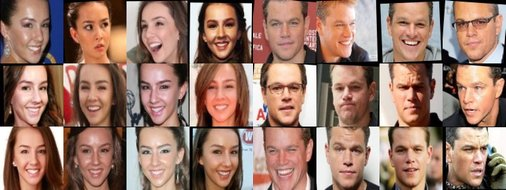
\includegraphics[width=3.2in]{FaceScrub.jpg}
  \end{flushright}
  \caption{Example Images from the FaceScrub Data Set}
\end{wrapfigure}

\noindent
For the re-ID of Humans, we consider the publicly available FaceScrub data set \cite{ng2014data} (Figure 1). This data set allows for a benchmark comparison of our methodology in comparison to other human similarity networks. After following the described data creation format, the training set contains 218,872 pairs of images, the validation set 21,231 pairs of images, and the test set 32,398 pairs of images created by considering 16 random individuals not included in the training data.  
\newline
\\
For the re-ID of Chimpanzee, I will consider the publicly available C-Zoo and C-Tai data sets introduced by Loos and Ernst (2013) combined into the \textit{Chimpface} dataset introduced by Deb et al (Figure 2). (2018) \cite{loos2013automated, deb2018face}. This data set provides the unique opportunity of comparing the performance of similarity comparison models to the previously reported performance of feature engineering as well as deep learning methods. After following the described data creation format, the training set contains 148,516 pairs of images, the validation set 13,656 pairs of images, and the test set 16,398 pairs of images created by considering 8 random individuals not included in the training data.  
\newline
\\
To test re-identifying Humpback Whales, I will consider the Humpback Whale Identification Challenge data set offered as a Kaggle competition \cite{kagglehumpbackreid}. This data set provides a realistic representation of the real world application of animal re-ID as the 9,046 images only contain the fluke of the whale and are extremely sparse, having only an average of only 2 (+/- 8) individuals considering 4,251 individual classifications (Figure 8). After creating the pairwise data, the training set has 25,399 image pairs, validation set 2,655 image pairs, and test set 3,822 image pairs. There are much fewer images because there are far less pair combinations for each individuals.
\newline

\begin{wrapfigure}{r}{0.5\textwidth}
  \begin{flushright}
    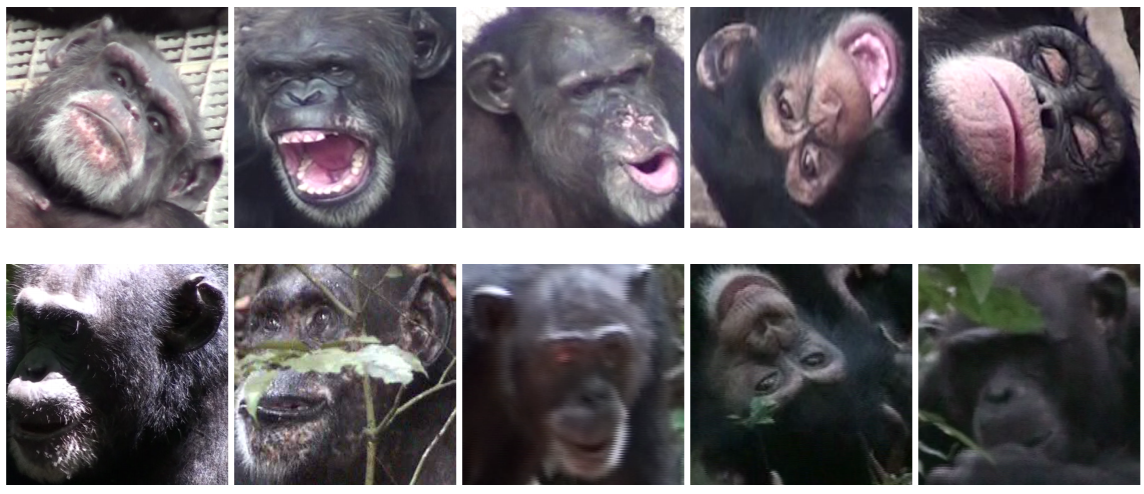
\includegraphics[width=3in]{ChimpanzeeExamples.png}
  \end{flushright}
  \caption{Example Images from the Chimpface Chimpanzee Data Set}
\end{wrapfigure}

\noindent
To test the re-ID of Fruit Flies, we collaborate John Schneider to test our similarity network on a large library of high resolution images of fruit flies \cite{schneider2018can} (Figure 3). The large number of images available here provide an excellent opportunity to test the capabilities of similarity learning networks on an animal species where re-ID is beyond the capabilities of a human observer. After following the described data creation format, the training set contains 216, 421 pairs of images, the validation set 23, 423 pairs of images, and the test set 17,632 pairs of images created by considering 4 random individuals not included in the training data.  
\newline

\begin{wrapfigure}{r}{0.6\textwidth}
  \begin{flushright}
    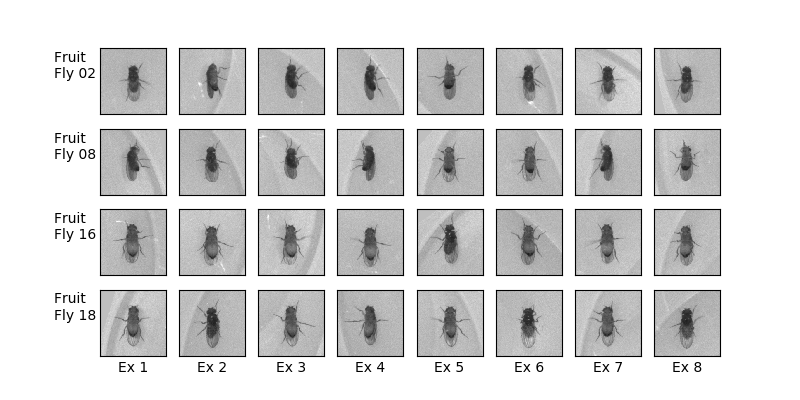
\includegraphics[width=4.2in]{FruitFlyExamples.png}
  \end{flushright}
  \caption{Example Images from the Fruit Fly Data Set}
\end{wrapfigure}

\noindent
Lastly, to test the re-ID capabilities considering octopus we consider a real world scenario where images are not readily curated into a data set, but instead extracted from video when multiple individuals are on screen \cite{scheel2017second}. This data set demonstrates the framework for real-world application as it requires an accurate object detector to identify octopus as they enter the video frame and a similarity comparison network to determine if these individuals has been previous seen before. Gathering the data required to train the object detector involves documenting the bounding box coordinates for each octopus in each frame of video to train the object detector as well as extract these isolated octopus images into labeled folders of unique individuals to train the similarity comparison network. An example of a trained a Faster R-CNN object detection model using the Inception architecture to localize octopus within an video sequence with 96.4\% accuracy can be found at: https://www.youtube.com/watch?v=TXbv5pN4JRI \cite{schneider2018deep}.
\newline
\\
To collect bounding box and extract images of octopus individuals, I have created a universally applicable video data extraction tool to streamline the process. The user begins by selecting their video of interest. The software then asks the user to place their mouse cursor at the top left corner of an object of interest (eg. octopus) and follow along while the video plays and it records the X\&Y position of the mouse cursor for every frame. The software then repeats the video for the user to follow the bottom right corner of the same object. The user can then select if there are additional objects and repeat/review the process until the video is fully labeled. The end result are the necessary files required for the two data formats: the bounding box coordinates per frame of each octopus individual used to train the object detector, and the extracted images of each octopus individual used to train the similarity network. A demo of this software is available at: https://youtu.be/YcTj0ayztA4 and is publicly available on GitHub at https://goo.gl/XomSao. 
\newline
\\
For our testing purposes, we labeled 16 short octopus videos with 3.5 average octopuses per video and an average length of 2:14 minutes. Three randomly selected videos are used to create the test set. We manually inspected each catalog of images and delete approximately 90\% of images that appear redundant over time (ie. when an octopus remains stationary). We then follow the same Siamese data creation format as listed above for each video independently to create a current total of 80,916 training pairs, 9,080 validation pairs, and 17,968 unseen testing pairs. Pairwise interactions are only considered within each video segment where the octopus remains on screen as the identity of individuals across videos is uncertain.

\section*{Animal Re-Identification Results}

Our network architecture follows the Siamese Network construct, composed of two sister networks where we implemented two VGG19 architectures, consisting of 13 2-dimensional convolution layers and 5 max pooling layers \cite{simonyan2014very}. The features of the last convolution layers are then concatenated together and passed through two 2048 node fully connected layers, and lastly through a binary output representing similar/dissimilar pairs. Details of the training process can be found in Appendix A.
\newline
\\
Considering the FaceScrub data set, the model produces a training set accuracy of 91.3\%, a validation accuracy of 91.3\%, and test set accuracy of individuals never seen during training of 89.7\%. Considering state of the art models, such as FaceNet, our model does not match their level of performance, however it does perform well enough to indicate their is room for improvement in terms of architecture, and demonstrate the capabilities of this system for animal re-ID. This serves a platform of comparison for how similarity learning models perform on a variety of difference species and data set composition. 
\newline

\begin{figure}
	\begin{center}
    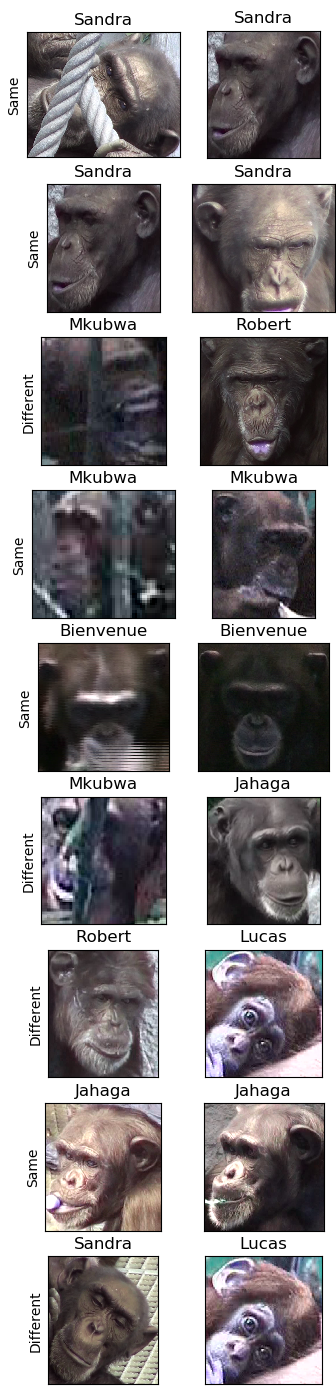
\includegraphics[width=2.0in]{ChimpanzeeComparison.png}
  \caption{Model Output for Chimpanzee Individuals. Y label for each image is the model output and the X label is the name of each individual in the below photo}
  	\end{center}
\end{figure}

\noindent
Considering the \textit{Chimpface} data set, the model produces a training set accuracy of 88.2\%, a validation accuracy of 87.5\%, and test set accuracy of individuals never seen during training of 75.5\%. This is a large improvement over the verification score of 59.9\% using the same data reported by Deb et al. (2018) \cite{deb2018face} (Figure 4 \& 5).
\newline
\\
Considering the humpback whale data set, the model returns a training set accuracy of 65.2\%, validation accuracy of 62.3\% and test accuracy of 61.4\%. A low training accuracy suggests either the model is not complex enough to capture the representation of whale individuals, which is unlikely considering its success on \textit{Chimpface}. As a result, we further data augmentation techniques may help improve performance further (Figure 6). While a poor result in comparison to acceptable standards for monitoring, while the competition has since expired, our approach currently stands as the 4th best performing model considering 528 entries. 
\newline
\\
For the fruit fly data set, the model returns a training set accuracy of 82.4\%, validation accuracy of 82.0\% and test accuracy of 79.3\%. While distinguishing between fruit fly individuals seems to be an impossible task for humans, our model was able to successfully learn features which accurately distinguish between individuals. Considering the data set, the success of this model is likely based on the very large number of training images available, as well as the standardized background of the images themselves.
\newline
\\
Considering the created octopus data set, the model returns a training accuracy of 97.8\%, validation accuracy of 95.3\% and testing accuracy of 92.2\% considering octopus it hasn't seen during training (Figure 7). These results show promise considering more data can still be collected. Pushing to achieve greater than 95\% accuracy seems like a tangible objective with additional image augmentation techniques. 
\newline
\\
A summary of results can be found in Table 1.

\section*{Near Future Techniques for Animal Re-Identification}
By considering modern deep learning approaches, ecologists can utilize improve accuracies without the requirement of hand-coded feature extraction methods by training a neural network from large amounts of data. The success of our models across multiple species and environments show that similarity learning networks are capable of solving the one-shot learning problem associated with animal population monitoring. 
\newline
\\
In practice, a wildlife re-ID system would work as follows. One would collect or find a data library of images of animal individuals for the species in consideration, ideally in the 1,000+. One would then organize the images into pairs and train a Siamese network to distinguish if two animal individuals are the same. In addition, one would train an object detector to localize the animal species from a camera trap image \cite{schneider2018deep}. Once both models are trained, one can set up the object detector to extract animal species from images which are then fed into the Siamese network. One can be used to estimate population sizes by querying a database. Upon initialization, this database would be empty. As each individual enters into the camera, the network will query each existing animals within the database. If none are deemed to be similar, an image of the new individual will be added to the database and the process repeats for each individual that enters. 
\newline
\\
In order for such technqiues to become generally applicable, we foresee the greatest challenge for deep learning methods being the creation of large 1,000+ labeled datasets for animal individuals. Our proposed approach for data collection would be to utilize environments with known ground truths for individuals, such as national parks, zoos, or camera traps in combination with individuals being tracked by GPS, to build the datasets. We would recommend using video wherever possible to gather the greatest number of images for a given encounter with an individual. We encourage researchers with images of labeled animal individuals to make these datasets publicly available to further the research in this field. In addition to gathering the images, labeling the data is then also a labourious task, especially when training an object detection model where bounding boxes are required. One approach for solving this problem is known as weakly supervised learning, where one provides object labels to a network (ie. zebra) and the network returns the predicted coordinates of its location \cite{zhou2017brief}. An alternative approach is to outsource the labeling task to online services, such as Zooniverse which can be time saving for researchers, but introduces inevitable error and variability \cite{simpson2014zooniverse}. 
\newline
\\
While deep learning approaches are able to generalize to examples similar to those seen during training, we foresee various environmental, positional, and timing related challenges. Environmental difficulties may include challenging weather conditions, such as heavy rain, or extreme lighting/shadows, especially from video analysis that only make comparisons between similar weather conditions. A possible solution to limit these concerns may be to re-ID only during optimal weather conditions. A second is to include a robust amount of image augmentation. A positional challenge may occur if an individual were to enter the camera frame at extremely near or far distances. To solve this, one could limit animals to a certain range from the camera before considering it for re-ID. Lastly, a challenge may be if an individual's appearance were to change dramatically between sightings, such as being injured or the rapid growth of a youth. While a network would be robust to such changes given training examples, this would require examples be available as training data. To account for this issue we would consider having a `human-in-the-loop' approach, where a human monitors results and relabels errorenous classifications for further training to improve performance \cite{holzinger2016interactive}. 
\newline
\\
While today fully autonomous re-ID is still in development, researchers can already use these systems to reduce manual labour for their studies. Examples include training networks to filter images by the presence/absence of animals, or species classifications \cite{kaggleiWildCam2018, norouzzadehautomatically, schneider2018deep}. Soon deep learning systems will accurately perform animal re-ID at which time one can create systems that autonomously extract from camera traps a variety of ecological metrics such as diversity, evenness, richness, relative abundance distribution, carrying capacity, and trophic function, contributing to overarching ecological interpretations of trophic interactions and population dynamics.

\section*{Conclusion}
Population estimates are the underlying metric for many fundamental ecological questions and rely on the accurate re-identification of animals. Camera and video data have become increasingly common due to their relatively inexpensive method of data collection, however they are criticized for their unreliability and bias towards animals with obvious markings. Feature engineering methods for computer vision have shown success re-identifying animal individuals and removing biases from these analyses, however these methods require algorithms designed for feature extraction. Deep learning provides a promising alternative for ecologists as it learns these features from large amounts and has shown success for human and animal re-ID. By utilizing deep learning methods for object detection and similarity comparison, ecologists can utilize deep learning methods to autonomously re-identify animal individuals from camera trap data. Our results here demonstrate how such a tool would allow ecologists to automate population estimates.
\newpage

\section*{Appendix A}

In addition to the general architecture, we consider a variety of regularization techniques to improve training stability and prevent overfitting. Initializing the model with the Xavier (also known as Glorot normal) initialization helps improve the likelihood of successful training over random initialization which often stays within a plateu with no gradient information \cite{glorot2010understanding}. Also, before each fully connected layers I implement batch normalization, a technique shown to help improve generalization of a model \cite{ioffe2015batch}. To prevent overfitting, I also regularize the final two fully connected layers with a Ridge regression value of 0.01 which penalizes the complexity of the function by including a squared error term that the model must also minimize \cite{hoerl1970ridge}. I also include a 50\% dropout for both fully connected layers which for each mini-batch randomly prohibits the use of 50\% of the nodes in the fully connected layers \cite{srivastava2014dropout}.
\newline
\\
In addition to these techniques, to help improve generalization I also apply data augmentation methods during training. For every training example, there is a given probability that the image will be modified in some capacity while maintaining the correct labels. This technique helps improve generalization and reduce overfitting as it artificially creates additional training examples. For each training example there is a random chance of noise to be added for colour channel manipulation, per pixel manipulation, bluriness, and pixel dropbout. Image Augmentation are performed using the ImgAug library \cite{imgaug}. 
\newline
\\
To train the weights of the neural network I select the Adaptive Momentum (Adam) optimizer with a learning rate of 0.001 \cite{kingma2014adam}. Simply stated, Adam is regarded as the most capable optimizer, able to increase and decrease its step size relevant to the speed at which the error is decreasing and also adjusting its direction travel to the steepest descent similar to the optimizer RMS Prop \cite{kingma2014adam}. To represent error, I consider the binary crossentropy loss considering the binary output of the similarity network. I train the model using mini-batch sizes of 128 training examples. As a metric for recording performance during training, I consider the accuracy on the test set of previously unseen individuals and only save the model if the current epoch is an improvement over the previous. In essence, this approach allows me to consider early stopping as a means of regularization and selects the model which best generalizes to unseen individuals. With the above considerations, I train the model for 100 epochs. Training and analyses of this model were performed using Python 3.6, Tensorflow 1.8, and Keras 2.2 using two GPUS: NVidia 1080 GTX and NVidia 680 GTX. 



\newpage
\begin{table}[h!]
\centering
\caption{Summary of Performance Metrics for Similarity Learning Models be Species \& Data Set}
\begin{tabular}{ l c c c c c c}
	\multicolumn{7}{ c }{}\\
	\hline
	Species & \multicolumn{1}{p{2cm}}{\centering Total\\ Images} & \multicolumn{1}{p{2cm}}{\centering Num.\\ Individuals} & \multicolumn{1}{p{2cm}}{\centering Avg. Num. Images /\\ Individual} & \multicolumn{1}{p{2cm}}{\centering Num. Pairs\\ Used for Training} & \multicolumn{1}{p{1cm}}{\centering Val.\\ Acc.} & \multicolumn{1}{p{1cm}}{\centering Test\\ Acc.} \\ \hline	
	Human & 65,943 & 530 & 127.3 & 218,872 & 91.3 & 89.7\\		
	Chimpanzee & 5, 599 & 90 & 71.0 & 148,516 & 87.5 & 75.5 \\
	Humpback Whale & 9,046 & 4,251 & 2.1 & 25,399 & 62.3 & 61.4 \\
	Fruit Fly & 244,760 & 20 & 12,238.0 & 218,872 & 82.0 & 79.3 \\
	Octopus & 5,192 & N/A & 92.7 & 80,916 & 95.3 & 92.2 \\
\end{tabular}
\end{table}


\newpage
\begin{table}[h!]
\centering
\caption{Summary of Performance Metrics for Parks Canada Species ID}
\begin{tabular}{ l c c c c }
	\multicolumn{5}{ c }{}\\
	\hline
	Model & 
	\multicolumn{1}{p{2cm}}{\centering Accuracy} & 
	\multicolumn{1}{p{2cm}}{\centering F1 Score} & 
	\multicolumn{1}{p{3cm}}{\centering ImageNet Top 1-Accuracy} & 
	\multicolumn{1}{p{2cm}}{\centering Model Size (MB)} \\ \hline	
	DenseNet201 & 0.813 & 0.505 & 0.773 & 80\\		
	Inception ResNetV2 & 0.819 & 0.428 & 0.803 & 215 \\
	InceptionV3 & 0.822 & 0.494 & 0.779 & 92\\
	MobileNetV2 & 0.867 & 0.636 & 0.713 & 14 \\
	VGG16 & 0.803 & 0.414 & 0.713 & 528 \\
	Xception & 0.841 & 0.477 & 0.790 & 88\\
\end{tabular}
\end{table}

\begin{figure}
    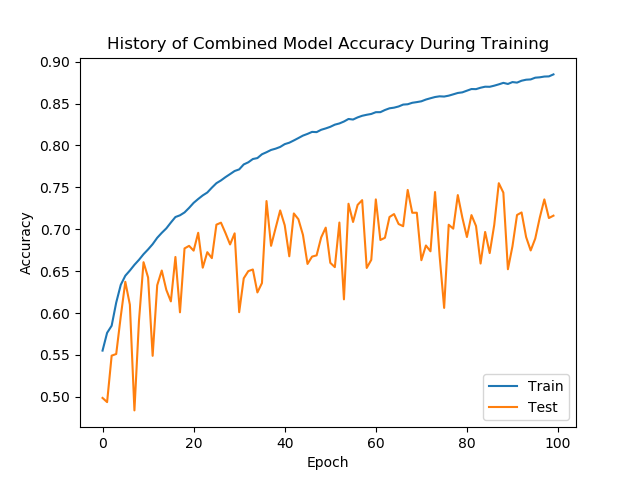
\includegraphics[width=17cm]{ChimpAcc.png}
  \caption{Chimpanzee Accuracy}
\end{figure}

\begin{figure}
    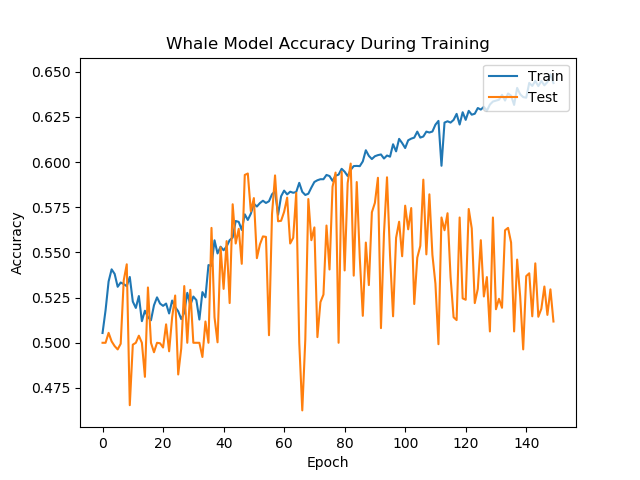
\includegraphics[width=17cm]{HumpbackWhaleAccuracy.png}
  \caption{Humpback Whale Accuracy}
\end{figure}

\begin{figure}
    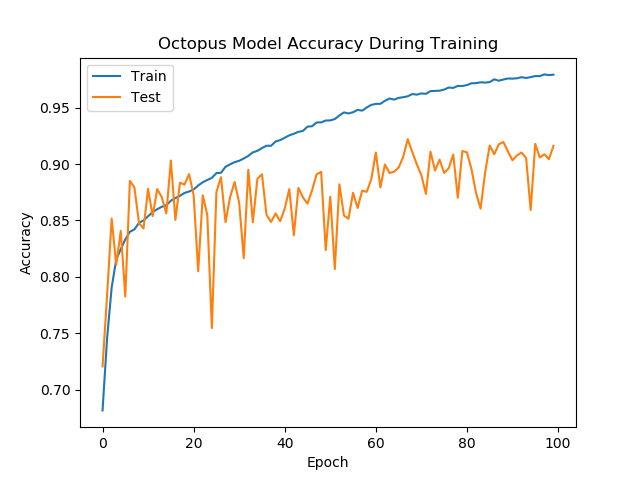
\includegraphics[width=17cm]{OctopusAccuracy.png}
  \caption{Octopus Accuracy}
\end{figure}



\clearpage
\bibliographystyle{IEEEtran}
\bibliography{MasterReference}

\end{document}

